\documentclass[a4paper,10pt]{report}
\usepackage[T1]{fontenc}
\usepackage[utf8]{inputenc}
\usepackage[frenchb]{babel}
\frenchbsetup{StandardLists=true}
\usepackage{enumitem}
\usepackage{lmodern}  % Pour changer le pack de police
\usepackage{makeidx}
\usepackage{circuitikz}
\usepackage{amsmath}
\usepackage{amssymb}
\usepackage{mathrsfs}
\usepackage{graphicx}
\usepackage{url}
\usepackage{array}
\newcolumntype{M}[1]{>{\raggedright}m{#1}}
\title{Rapport travail 1 \\EZMeal}
\author{Groupe R\\ \\Jean-Benoit Berlier\\Laurent Desausoi \\ Martin Fockedey \\Maxime Mawait \\Arthur Van Stratum 
}
\date{\today}
\makeindex

\begin{document}
\begin{titlepage}
\begin{figure}[t]

\includegraphics[scale=0.3]{epl-logo.jpg}
\end{figure}

\maketitle 

\end{titlepage}

\tableofcontents

\pagebreak

\chapter{Avant-propos}

Dans le cadre du cours de conception orientee objet, il nous a ete demande de realiser une application de cuisine pour une chaine de supermarches: "EZMeal".
Ce document reprend les differents choix de conception effectue lors de la conception du schema ORM et des bases de donnees liees.

\begin{figure}[!h]
	\center
	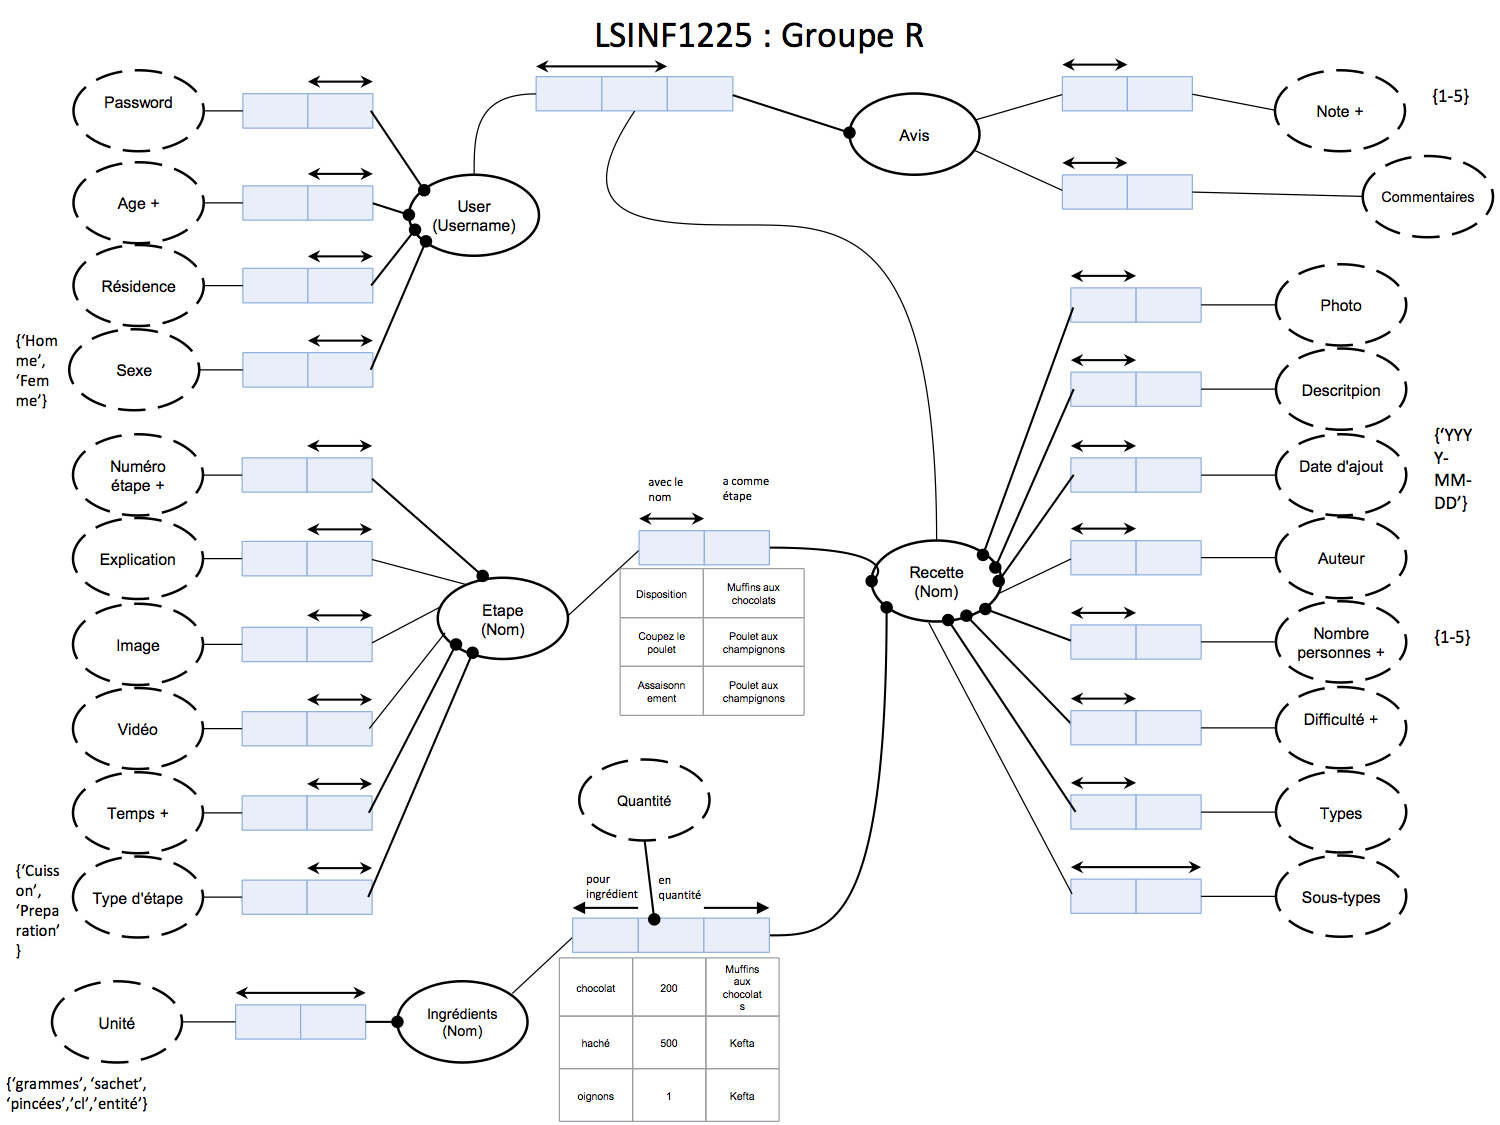
\includegraphics[scale = 0.25]{SchemaORM.jpg}
	\caption{Schema ORM de l'application EZMeal}
	\label{ORM}
\end{figure}

\pagebreak

\chapter{Conception et contenu des differents tableaux}

La base de donnees et l'application sont organisees autour de six tableaux differents (Utilisateurs, Recette, Avis, Etape, Unite d'ingredients et Ingredients), regroupant chacun un nombre variable de champs.  La base de donnees est construite de telle sorte a ce qu'il y ait un maximum de relations binaires et le moins de relations ternaires.

\section{Utilisateurs}

Ce tableau est un element principal de cette application car il stocke les donnees personnelles et interactions sur l'application en memoire. Ce tableau presente un leger inconvenient. En effet, il existe une relation ternaire entre ce tableau et les tableaux recette et avis.

Le tableau contient les champs suivants:
\begin{itemize}
	\item Username, ce champ est le champ principal du tableau. Nous l'avons choisi comme tel car nous trouvons que c'est la maniere la plus adequate de qualifier un utilisateur. Ce champ est unique pour un utilisateur car c'est ce qui caracterise un utilisateur.
	\item Password, ce champ est obligatoire et unique pour un utilisateur donne. pour des raisons de securite.
	\item Age, ce champ est obligatoire et unique pour un utilisateur. Ces deux conditions sur la relation sont specifiees dans le canevas de l'application.
	\item Residence, ce champ est obligatoire et unique pour un utilisateur. Ces deux conditions sur la relation sont specifiees dans le canevas de l'application.
	\item Sexe, ce champ est obligatoire et unique pour un utilisateur. Ces deux conditions sur la relation sont specifiees dans le canevas de l'application.
	\end{itemize}
\section{Avis}

Ce tableau n'est pas l'extension qui nous devons implementer. C'est un choix purement subjectif d'extension supplementaire a faire car nous nous sommes dits que ce serait mieux pour l'experience utilisateur de pouvoir communiquer sur les recettes, emettre son avis et des conseils/ajustements sur la recette. Le principal desinconvenient de ce tableau est le fait qu'il y ait une relation ternaire entre ce tableau et les tableaux recette et utilisateur.

Le tableau contient les champs suivants:
\begin{itemize}
	\item Username, ce champ est obligatoire et unique car chaque avis doit avoir un auteur.
	\item Note, ce champ n'est pas obligatoire mais est unique pour un avis car nous pensons que, pour un avis, il n'est pas obligatoire de donner une note mais chaque avis ne peut contenir qu'une seule note.
	\item Commentaires, ce champ n'est pas obligatoire et n'est pas unique car un avis peut contenir plusieurs commentaires mais n'est pas obligatoirement rempli.
	\item Recette, ce champ est unique et obligatoire car chaque avis doit porter sur une recette.
\end{itemize}

\section{Recette}

Ce tableau est l'element principal de l'application. En effet, ce tableau est connecte a tous les autres tableaux et l'application est principalement base sur cette base de donnees. Cependant, ce tableau a une relation ternaire avec les tableaux utilisateur et avis et une avec quantite et ingredients.

\begin{itemize}
	\item Nom de la recette, ce champ est obligatoire et est la cle primaire de ce tableau car c'est la maniere la plus conventionnelle de caracteriser une recette. 
	\item Description, ce champ est obligatoire car c'est extremement utile d'avoir une petite description pour la recette pour choisir la recette a cuisiner.
	\item Photo, ce champ est obligatoire car les images de recettes sont un facteur tres important pour se faire une idee de la recette et dans la majorite des cas, une photo appetissante  va encourager l'utilisateur a choisir cette recette.
	\item Date d'ajout, ce champ est obligatoire car chaque recette a une date d'ajout.
	\item Auteur, ce champ est obligatoire car chaque recette a un auteur.
	\item Nombre personnes, ce champ est obligatoire car il est important dans son choix de recettes de savoir pour combien de personnes cette recette est destinee.
	\item Difficulte, ce champ est obligatoire car, pour un novice, il est extremement important de ne pas prendre une recette difficile a cuisiner.
	\item Types, ce champ est obligatoire car c'est toujours de cuisiner un plat et non un dessert pour le plat de resistance.
	\item Sous-types, ce champ n'est pas obligatoire car ce champ est purement instructif et utile pour les recherches car c'est utile si on veut chercher un plat italien par exemple.
\end{itemize}

\section{Etape}

Ce tableau est un element determinant de notre application car il s'agit de notre extension imposee. De plus, ce tableau est tres important pour l'experience utilisateur car il apporte plus d'explications a une recette, ce qui peut moins decourager les utilisateurs a cuisiner.

\begin{itemize}
	\item Nom de la recette,  ce champ est obligatoire et est la cle primaire de ce tableau car ce tableau se rapporte a des recettes qui sont caracterisees par leur nom.
	\item Nom de l'etape,  ce champ est obligatoire car c'est ce qui caracterise l'etape.
	\item Explication, ce champ n'est pas obligatoire car toutes les etapes n'ont pas besoin d'explication. (cfr: couper des patates)
	\item Image, ce champ n'est pas obligatoire car toutes les etapes n'ont pas besoin d'images d'explication. (cfr: couper des patates)
	\item Video, ce champ n'est pas obligatoire car toutes les etapes n'ont pas besoin de videos d'explication. (cfr: couper des patates)
	\item Temps, ce champ est obligatoire car chaque a un temps de preparation.
	\item Type d'etapes, ce champ est obligatoire car chaque etape a un type qu'il est interressant de connaitre. (cfr: cuisson) 
\end{itemize}

\section{Ingredients}

Ce tableau est important car, sans ingredients et sans une quantite precise de ces ingredients, une recette est impossible a executer. Ce tableau est specifique a une recette car il reprend la quantite necessaire de cet ingredient dans la recette.

\begin{itemize}
	\item Nom de la recette, ce champ est obligatoire car chaque ingredient convient a une recette.
	\item Nom de l'ingredient, ce champ est obligatoire car chaque ingredient a un nom.
	\item Quantite, ce champ est obligatoire car c'est le champ qui determine l'utilite de ce tableau.
\end{itemize}

\section{Unites des ingredients}

Ce tableau est important car c'est un tableau generique reprend la facon dont mesure chaque ingredient.

\begin{itemize}
	\item Nom de l'ingredient, ce champ est obligatoire et est la cle primaire de ce tableau car c'est ce qui caracterise le mieux ce tableau.
	\item Unite, ce champ est obligatoire car chaque ingredient a une methode de mesure differente.
\end{itemize}

\end{document}
